\section{Data Analysis}
\subsection{Testing the Causal Model}
\todo{Give algorithm for the onpass scenario.}

\c2j{}{\subsection{Experimental Setup}\label{sec:setup}}
As mentioned, we used \azdb\ to run the experiments. This infrastructure,
now comprising about 45K lines of code, handles all the details of
generating the sample data, generating the actual queries, collecting the
various plans generated by the optimizer, running the queries, and storing
the results in a ``lab notebook,'' a set of tables managed by
a separate DBMS. This infrastructure also performs the many steps
required to ensure repeatability.

We have assembled a hardware lab of dedicated
machines, one \c2j{for each DBMS}{each for the three DBMSes} and one to run the DBMS used
to store the lab notebooks. Having dedicated hardware allows us to worry
less about other processes running on the machines that could dirty the
results (these machines are {\em only} for experiments), and allows us to
run extensive experiments involving days or weeks of computation. We have
used this software and hardware lab to perform a number of experiments
examining the phenomenon of suboptimality.

\azdb\ utilizes experiments defined in XML. It supports {\em experimental
  scenarios}, which are short (perhaps 100 lines of code) Java subclasses
that provide details of how to run kinds of experiments.

In the following, we describe in detail the data used by our experiments and
the experimental \c2j{scenario we utilized.}{scenarios we defined.}

\subsection{Datasets}\label{sec:datasets}
We generate our experiment datasets randomly in the experiments. However, we
use seeds to control the random data generator so that it can produce
repeatable data as required.

Our experiment datasets consist of relational tables. There are two types of
tables. The first is a ``fixed table'' that, once created and
populated, will never be modified in the future.  In contrast, the second
type is a ``variable table.'' We alter the cardinality\c2j{ statistics of
  this table}{, either physically or
virtually, of such tables} as the experiments are being performed. We will
elaborate the detailed discussion on modifying table cardinality
\c2j{statistics }{}when we
examine our experiment \c2j{scenario}{scenarios}.

\c2j{We used a}{We organized three configurations for the datasets. The first configuration
is a small} dataset with four tables, each with four integer-typed
columns. Each table is populated with one million rows. The size of each
table is roughly 16MByte ( =4 (bytes)$\times 4 \times$1,000,000).\c2j{}{ Second, to
perform queries with more relations, we create eight tables. In this case,
each table has the same configuration as in the first dataset. Third, to
test queries on large tables, we configure each table with 64 integer-typed
columns. In this dataset, we create four tables, but the size of each one is
512MByte.}

\shorten{\begin{figure*}[t]
\begin{center}
\begin{algorithmic}
{\bf Algorithm} generateQueries({\em numQueries}, %\\
%\quad
{\em maxNumCorrNames}, {\em maxNumColumns}, {\em whereAttributes}, {\em tableMetaData}):
\FOR{$i$ $\leftarrow$ 1 {\bf to} {\em numQueries}}
\STATE    {\em numCorrNames}       $\leftarrow$ random(1, {\em maxNumCorrNames})
\STATE    {\em numColumns}      $\leftarrow$ random(1, {\em maxNumColumns})
\STATE    {\em corrNames}	$\leftarrow$ getCorrNames({\em numCorrNames})
	\FOR{$j$ $\leftarrow$ 1 {\bf to} {\em numCorrNames}}
	\STATE	{\em tableNames}[$j$]	$\leftarrow$ {\em tableMetaData}[random(1, %\\
%\hspace*{2in}
{\em tableMetaData}.numTables)].tableName
	\ENDFOR
	\FOR{$j$ $\leftarrow$ 1 {\bf to} {\em numColumns}}
	\STATE	{\em columnNames}[$j$]	$\leftarrow$ pickColumn({\em corrNames}, %\\
%\hspace*{1.5in} 
{\em tableMetaData})
	\ENDFOR
\STATE    {\em selectClause}   $\leftarrow$ generateSelectClause({\em columnNames})
\STATE    {\em fromClause}     $\leftarrow$ generateFromClause({\em tableNames}, %\\
%\hspace*{1.5in}
{\em corrNames})
\STATE    {\em whereClause}    $\leftarrow$ generateWhereClause({\em tableNames}, %\\
%\hspace*{1.5in}
{\em corrNames}, {\em whereAttributes})
\STATE    {\em queries}[$i$]      $\leftarrow$ {\em selectClause} + {\em fromClause} + {\em whereClause}
\ENDFOR
\STATE {\bf return} {\em queries}
\end{algorithmic}
\caption{Algorithm for Random Query Generation\label{alg:querygen}}
\end{center}
\end{figure*}

The XML specification of the \c2j{dataset}{first dataset (the others are similarly
specified)} is shown in Figure~\ref{fig:expspec}. Note that we do not specify any
constraints such as primary keys and foreign keys, nor did we specify
primary or secondary indexes. This will have the impact of eliminating
several operators which might be used in plan generation, such as index
scan. Interestingly, even though the data and query complexity are both
quite restricted (though we can vary query complexity \c2j{somewhat}{through
  our three datasets}), we still observed suboptimality\c2j{}{ in all three of our subject DBMSes}.

The experimental specification also configures the randomly generated
queries. The query specification stated that 500 queries were to be
generated\c2j{}{; this set of queries were generated for the first experimental
subject and then used with the other two experimental subjects}. Each query
is a simple select-project-join (SPJ) query, with a few attributes in the
SELECT clause, a few tables referenced in the FROM clause, and a few
equality predicates in the WHERE clause. As such some of the complexities
mentioned by Kabra and DeWitt~\cite{kabra98}, such as
user-defined data types, methods, and operators, are not considered.  The queries were generated
by a simple algorithm, the pseudo-code for which is shown in
Figure~\ref{alg:querygen}.

The query generator has three main components, which are {\tt
  generateSelectClause()}, {\tt generateFromClause()}, and {\tt
  generateWhereClause()}. The select clause will contain from one to four
columns\c2j{}{, hence, an average of 2.5 columns}. The number of correlation names
in the FROM clause varied from one to four, with duplication of tables
allowed (duplicate table names within a from clause implies a self-join).
In the queries that were generated, from one to four unique tables were
mentioned in the FROM clause. Somewhat fewer tables were mentioned than the
number of correlation names, as the presence of self-joins reduced the
number of unique tables named by the queries.

In {\tt generateWhereClause()}, in which all the joins will appear, we make
sure that Cartesian products are
eliminated\c2j{.}{(\verb.cartesianPossible="false".)}  We do this by
connecting all the correlation names that appear in the FROM statement via
comparisons on random columns. In this case, the comparisons are all
equality operators. To ensure that the queries are as simple as possible, we
do not include any additional predicates in the WHERE clause.  \c2j{}{This
  is realized by setting the attributes {\tt maxIsAbsolute} to {\tt true}
  and {\tt complexUsePercentage} to {\tt 100}.  Basically, ``complex''
  predicates eliminate the Cartesian product, and by setting complex
  predicates as ``absolute,'' no additional predicates are included except
  for those which are necessary for eliminating Cartesian product.} Also for
simplicity, we do not include disjunctions nor negations.

\c2j{}{The settings of the query parameters are related to the definition of the test
tables. For example, the experiment involving eight tables would expect the
queries to be generated also have the appearance of the eight tables (at most).
}
}

\todo{ Add discussion of exhaustive, onepass}

\subsection{Data Analysis}\label{sec:dataanalysis}
\todo{Include details of how many queries, plans were selected and how many runs across how many DBMSes to illustrate complexity. }
\todo{Discuss statistics in more detail. }
Through many weeks of testing, we were able to eliminate the caching and
buffering artifacts via five general steps.  First, we cleared the DBMS
buffer via the provided API, to discard cached content residing inside
the DBMS. \c2j{}{(In some cases, there were multiple caches to be cleared, each
with a different kind of command. As mentioned above, these caches were
often not clearly documented.) }Second, we flushed the OS-related
caches.\c2j{}{ Under our experimental system, which is Linux, we used the {\tt
  drop\_cache} facility to discard cached clean pages from
cache. Considering that in query plan generation, no dirty pages would
necessarily be involved, clearing the clean page is sufficient.} Third, we
filled the on-disk cache, which is resident on the hard-drive, by reading a
data file of size 64MB. The size of the data file was chosen such that it is
bigger than the hard-drive buffer, which is 32MB. Fourth, we disabled,
through a variety of means, over a
dozen daemons that were not needed on a dedicated server. The final step
disabled, again, in various ways, some of the daemons running within the DBMS.
Through all of these
efforts in concert, we were able to obtain quite stable and repeatable
measurements of the time each plan for each query executed. Skipping any
one of these steps adds significant variability to the timing of a query.

There was still some residual variability in the timing of the execution
plans for each query. We have evidence that this variability is due to DBMS
daemons that occasionally wake up and expend system resources for a second
or two, sometimes more. (While we were able to disable or stop some of the
DBMS daemons, others seemed to be required by the DBMS for correct execution or
could not be disabled or delayed.) To get a handle on this variability, we ran some
experiments several times and compared the times.  Out of 100 queries that
were run, with multiple plans for each, each set run eleven times
independently, we found that the times were tightly clustered around the
median time, with some outliers, either where one or more daemon(s) happened
not to run during that query or where one or more daemons ran more often or
longer than normal during that query.

To understand the variability (and thus the repeatability) of these timings,
we plot in Figure~\ref{fig:stddev} the distribution of the four measured
times around the median time for that plan, eliminating the three lowest and
highest times (hence, we are considering the two times immediately below and
above the median). The $x$-axis is in terms of percentage of the
median. Each plan took around 5 seconds (the fastest plan took 0.3 seconds,
the slowest, 527 seconds, for different queries...). A standard deviation of
2.73\% indicates that 95\% of the plans were within (above or below) an
average of 140msec of the median.

\begin{figure}[bth]\centering
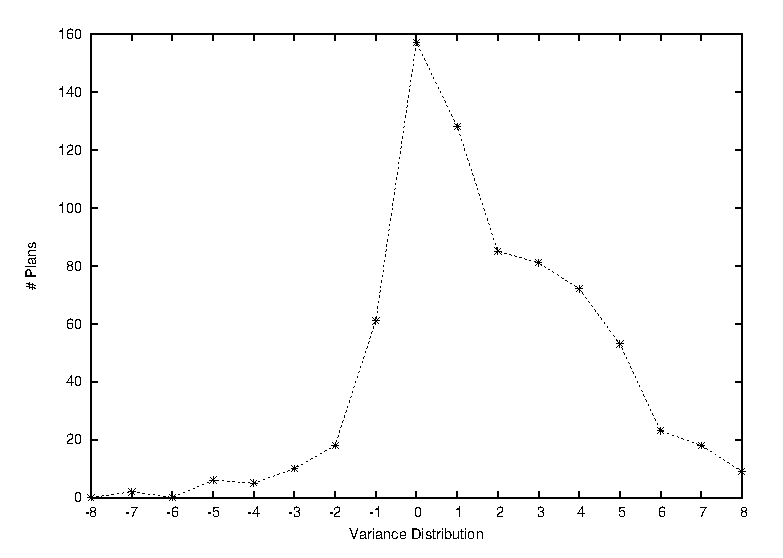
\includegraphics[width=0.50\textwidth]{figures/variance_distribution.eps}
\caption{Distribution of plan timings around the median\label{fig:stddev}}
\end{figure}

Our experimental timing methodology emerged from this initial data. We ran each
plan of each query five times, clearing all the caches before each
execution. We then selected the median time out of these five runs. We
judged a plan~$A$ to be faster than a plan $B$, for the same query, if the
measured execution time of plan 
$A$, $t_A < 0.9454 \cdot t_B$, that is, if it is more than two standard deviations faster. If the query optimizer picked plan $B$ and
there existed such a faster plan~$A$, we marked the query as suboptimal. As an
additional check of the methodology, we randomly selected five sets of five
runs from the set of eleven runs of 100 queries discussed above. For each of
the five sets, we identified the suboptimal queries in each run. The number
of such queries differed by a total of only two queries across all five sets.

\comment{, perhaps
ten executions were extreme outliers; these plans were omitted from further
analysis. We then examined the remaining plans. We believe that the smallest
values is the accurate one since intuitively the execution of that
particular run suffered the least from other system activities. We then
normalized each run to its minimum value and computed the standard deviation
from that value to arrive at a relative threshold that we could use when
testing the hypotheses, as described in later sections.

For DBMS {\bf A}, the relative threshold was 0.169. For DBMS {\bf B}, that
value was 0.138. It was reassuring that these were quite similar, as the
underlying casual factors are likely to be similar. We did not have
sufficient data to compute the threshold for DBMS {\bf C}, and so used the
higher value, 0.169. We will use this threshold later to help
reduce the false positive instances in determining suboptimality.}

\begin{figure}[t]
\begin{center}
\begin{algorithmic}
{\bf Algorithm} executeSpecificExperiment($experimentSpec$):
\STATE initializeLabNotebookContent()
\STATE initializeExperimentTables()
\FOR{$phase$ $\leftarrow$ 1 {\bf to} getNumPhases()}
\STATE stepA($phase$, $varTables$)
  \FOR{$q$ $\in$ getExperimentRunQueries()}
    \IF{$q$ has result}
      \STATE getResultFromLabNotebook($q$)
    \ELSIF{checkToBePaused()}
      \RETURN false
    \ELSE
      \STATE storeQueryResult(analyzeQuery($phase$, $q$, \\
      \hspace{47.0mm}$experimentSpec$))
    \ENDIF
  \ENDFOR
\ENDFOR
\RETURN true
\end{algorithmic}
\caption{Algorithm for Executing a Specific Experiment\label{alg:exeSpecExp}}
\end{center}
\end{figure}

\begin{figure}[t]
\begin{center}
\begin{algorithmic}
{\bf Algorithm} analyzeQuery($phase$, $q$, $experimentSpec$):
  RecordedQueryRuns
\IF{$phase$ = 1}
  \STATE $plan$ $\leftarrow$ getQueryPlan($q.sql$)
  \STATE storeOptimalQueryRun($plan$, stepB($phase$, $plan$))
\ENDIF
\RETURN recordAllQueryRuns(\\
\hspace{18.0mm}findQueryRuns($phase$, $q$, $experimentSpec$))
\end{algorithmic}
\caption{Algorithm for Analyzing a Query\label{alg:analyzeQuery}}
\end{center}
\end{figure}

\begin{figure}[t]
\begin{center}
\begin{algorithmic}
{\bf Algorithm} findQueryRuns($phase$, $q$, $experimentSpec$):
  QueryRunResult
\STATE $queryRunResult$ $\leftarrow$ $\Phi$
\FOR{$cardinality$ $\in$ \\
\hspace{5.0mm}generateCandidateCardinality($experimentSpec$)}
\IF{$\lnot$ stepC($phase$, $varTables$, $cardinality$)}
  \RETURN queryRunResult
\ENDIF
\STATE $newPlan$ $\leftarrow$ getQueryPlan($q.sql$)
\IF{($newPlan$ is subopt plan in the first phase $\wedge$ \\
\hspace{8.0mm} $newPlan$ has {\em NOT} been executed) \\
\hspace{3.0mm} $\vee$ $newPlan$ is different from the previous plan}
  \STATE $queryRunResult$ $\bigcup$ stepD($phase$, $q.sql$, \\
  \hspace{40.0mm} $cardinality$))
\ENDIF
\ENDFOR
\RETURN $queryRunResult$
\end{algorithmic}
\caption{Algorithm for Finding Query Runs\label{alg:findQueryRuns}}
\end{center}
\end{figure}

\c2j{}{\subsection{Experimental Scenarios}}
\c2j{Experiment scenarios use the {\em Template Pattern}~\cite{gamma95} to
  control their variability.}{As discussed in Section~\ref{sec:subopt}, we used two approaches to
determine which queries were suboptimal. These were expressed as two
experimental scenarios named ``VaryStats'' and ``Upper.'' We used the
{\em Template Pattern}~\cite{gamma95} to ensure that the commonality between
these two approaches was explicit.} Specifically, we implemented
an abstract class with several methods \c2j{and, for the purpose of this
  study, one concrete subclass, defining a specific scenario}{and concrete
  subclasses, each defining one of the specific scenarios} through the definition of five
short methods, namely {\tt stepA()}, {\tt stepB()}, {\tt stepC()},
{\tt stepD()}, and {\tt getNumPhases()}. The abstract class provides the
{\tt execute\-SpecificExperiment()}
method (Figure~\ref{alg:exeSpecExp}) along with two helper methods,
{\tt analyze\-Query()} (Figure~\ref{alg:analyzeQuery}) and {\tt findQuery\-Runs()}
(Figure~\ref{alg:findQueryRuns}). \c2j{Each scenario iterates}{Both scenarios iterate} through the
queries, analyzing each one. (Through \azdb, a long-running
experi\-ment, which may take a week or more, can be paused and
restarted.) Most of the work is done in {\tt findQuery\-Runs()}, with the
execution tailored by the individual steps provided by the concrete scenarios.

The ``VaryStats'' scenario produces different plans by changing the
statistics of the variable table.  However, the {\em actual} cardinality of
the varying table remains at 1M rows. Each plan is thus run on the identical
set of tables. 

In this scenario, sub-optimality is defined by the existence
of a plan, produced at a non-actual table cardinality, that runs with a
shorter elapsed-time than the ``optimal'' plan chosen and executed at the
(same) actual cardinality. {\tt stepA} populates the variable table. {\tt
  stepB} times the execution plan for the actual table size and returns
statistics on that execution. {\tt stepC} changes the cardinality statistics
of the variable table and always returns true. {\tt stepD} times the plan
for the specified cardinality, which was set by the previous step.

\c2j{}{The ``Upper'' scenario is used when a DBMS does not allow the statistics to
be changed. This scenario simply executes the query by successively changing
the cardinality of the varying table, by starting at the maximum and
deleting tuples. Periodically (every 10K tuples deleted), the query is
optimized, and run whenever the plan changes. In this scenario, a more
conservative definition of suboptimality is used. Suboptimality is defined
by the existence of a plan, produced with a larger varying table table
cardinality, that still runs with a shorter elapsed-time than the
``optimal'' plan chosen and executed at the actual cardinality.

For this scenario, {\tt stepA} again populates the variable table and {\tt
  stepB} times the execution plan for the actual table size and returns
statistics on that execution. {\tt stepC} actually changes the variable
table by deleting rows; it returns false if the requested cardinality is
less than the actual cardinality (hence the name of the scenario: Upper).
As before, {\tt stepD} times the plan
for the specified cardinality, which was set by the previous step.
Note that this scenario avoids some of the complexities mentioned
by Kabra and DeWitt~\cite{kabra98}, as the statistics on the underlying tables are
completely accurate and the amount of available resources are known (only
the one query is run at a time) and the values of host language variables
are also known (the system configuration remains fixed as the queries are
optimized and then immediately evaluated.

\todo{Show same query in upper with changepoints. }

The idea is that the faster query on the larger table would run even faster
if executed on the table with the actual cardinality. We formalize this
assumption as follows.

\noindent
{\bf Definition:} {\em Monotonicity}: given a query $Q$ and an actual
cardinality $a$,

\quad\quad\quad$\forall p \in \hbox{\em plans} (p) \;\forall c > a \;( \hbox{\em time} (p,
c) \geq \hbox{\em time} (p,a) )$

\noindent
where {\em plans}($p$) is the set of plans generated by the optimizer and
{\em time}($p$, $c$) is the execution time of plan $p$ on the data set with
the varying table at cardinality $c$.Given the variability discussed in
Section~\ref{sec:dataanalysis}, we augment this definition with a threshold
$\sigma$,

\quad\quad\quad$\forall p \in \hbox{\em plans} (p) \;\forall c > a \;( \hbox{\em time} (p,
c) \geq \hbox{\em time} (p,a) )$

\hfill$\blacksquare$

To test this assumption, we counted the number of queries, out of the total
of 1000 queries, applying the above definition of a monotonic query. We
examined every case where the same plan was run at least two times, at
different varying cardinalities. Note that for some queries, multiple plans
were each run more than one. \todo{true?} We
expect that there should be no non-monotonic queries. The results of this
analysis is in Table~\ref{tab:monotonic}.

\begin{table}
\caption{\label{tab:monotonic}}
\end{table}

\todo{discussion}

Given this analysis, we can now use the Upper scenario as a more
conservative proxy for the suboptimality observed directly in the
VaryStats scenario. In the remainder, we will presents results for the
Upper scenario for DBMSes {\bf A}, {\bf B}, and {\bf C}. When appropriate,
we will also present results for the VaryStats scenario for DBMS {\bf A}.

\todo{some general discussion about the presence of suboptimal, and give the
graph of the time difference between the fastest plan and ``optimal'' plan.
\comment{\begin{figure}[t]
\centering
%originally 30pc
\epsfig{figure=vldb_figures/figure10/figure10.eps,width=20pc}
\caption{Difference in Execution Time between Chosen Plan and Fastest Plan\label{fig:diff}}
\end{figure}
}

Several initial conclusions can be drawn from this experiment, which was the
initial result of several semesters of programming effort and many days of
experimental runs. First, {\em every} DBMS exhibits suboptimality. Thus, this
phenomenon is likely to be a fundamental aspect of either the algorithm
(cost-based optimization) or the creator of the algorithm (human information
processing). Our theory includes both effects.}

\subsection{Validity of Upper Scenario}
Between the two categories of suboptimality, the {\em VaryStats}
scenario directly shows whether the plan selected for the actual cardinality
is optimal.  However, the {\em Upper} scenario relies on the monotonicity
assumption, which we showed holds. Therefore, we expect that the set of
queries observed with suboptimality in the {\em Upper} scenario is a subset
of the set of suboptimal queries in the {\em VaryStats} scenario. In
practice, due to the measurement variation in experiments, there exist
exception instances. Nevertheless, we determine for each scenario a proper
variation threshold by which most exceptions or false positive
suboptimalities can be eliminated. Thus, we expect that the suboptimality
set in ``Upper'' scenario is a very {\em close} subset of the one in
``Suboptimal'' scenario.

Figure~\ref{fig:mono_check} {\todo Draw figure}shows the percentage of suboptimality with various
variation threshold for both ``Upper'' and ``VaryStats'' scenarios. Note that
we choose for each scenario the threshold value at the obvious turning position
of the curves in that we believe that is where most the false positive 
suboptimality is filtered out. Table~\ref{tab:mono_check} demonstrates the
actual queries in the two suboptimality sets. {\todo what can be seen? }
}

